\documentclass[paper=a4,fontsize=11pt]{article}
\usepackage{amsmath,amssymb,amsthm}
\usepackage[protrusion=true,expansion=true]{microtype}	
\usepackage{algorithm}
\usepackage{algpseudocode}
\usepackage[margin=1.5in]{geometry}
\usepackage{graphicx}
\setlength{\textfloatsep}{0.1cm}
\setlength{\floatsep}{0.1cm}
\begin{document}
\title{TCSS 343 - Assignment 3}
\author{Jake McKenzie}
\maketitle
In this problem use the Master Theorem to find and prove tight bounds for these recurrences (6 points each).\\\\
To solve this problem I used the master theorem taken from CLRS. I used a bit of a stronger statement than what was stated in the theorem but they are equivalent mathematically due to the nature of limits. I will include the theorem for the reader's benefit. To check my work I decided to include what I obtained using the Akra-Bazzi method.\\
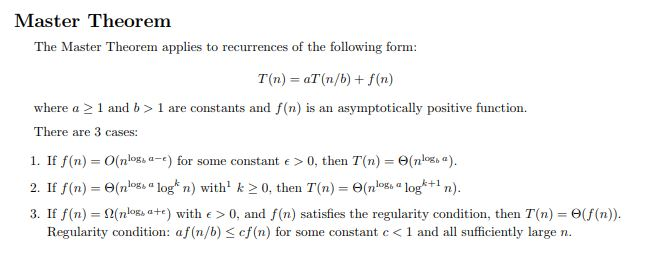
\includegraphics[width=\linewidth]{mastertheorem.JPG}
\begin{enumerate}
\item
\[
T(n) = \left\{
\begin{array}{cl}
c & \textrm{ if } n < 8\\
16T(n/8) + n\log{n} & \textrm{ if } n \geq 8
\end{array}
\right.
\]
\begin{align*}
\lim_{n\to\infty}\lim_{\varepsilon\to0}{\frac{n\log{n}}{n^{\log_{8}{16}+\varepsilon}}}&=\lim_{n\to\infty}\lim_{\varepsilon\to0}{\frac{n\log{n}}{n^{\frac{4}{3}+\varepsilon}}}\\
&=\lim_{n\to\infty}\lim_{\varepsilon\to0}{(\frac{n}{n})(\frac{\log{n}}{n^{\frac{1}{3}}n^{\varepsilon}})}\\
&=\lim_{n\to\infty}{(1)(\frac{\log{n}}{\sqrt[3]{n}(1)})}\\
&=\lim_{n\to\infty}{\frac{\log{n}}{\sqrt[3]{n}}}\rightarrow0\\
\end{align*}
From Knuth's concrete mathematics I know that any polynomial, even fractional powers, grows asytotically faster than a logarithm so this limit goes to 0. We have that problem one is the first case:
$$T(n)\in\Theta(n^{\frac{4}{3}})$$\\
By Akra-Bazzi I obtain:\\
\begin{align*}
16(1/8)^{p}&=1\\
p&=\frac{4}{3}\\
T(n) &= \Theta(n^{p}(1+\int_{1}^{n}{\frac{u\log{u}}{u^{p+1}}du}))\\
\end{align*}
\end{enumerate}
\end{document}